% % def.tex

% File containing LaTeX macros.
% Has grown by accretion; can be better organized.

\documentclass{article}
\usepackage{amsmath}
\usepackage{amssymb}
\usepackage{bm}
\usepackage{graphicx}
\usepackage{epstopdf}
\DeclareGraphicsRule{.tif}{png}{.png}{`convert #1 `basename #1 .tif`.png}
\usepackage{color}
\usepackage{pdfsync}
\pagestyle{plain}

%\pagestyle{empty}

\textheight 9 true in
\textwidth 6.5 true in
\hoffset -.75 true in
\voffset -.75 true in
 \mathsurround=2pt  \parskip=2pt
\def\crv{\cr\noalign{\vskip7pt}}

\def\a{\alpha } \def\b{\beta } \def\d{\delta } \def\D{\Delta } \def\e{\epsilon }
\def\g{\gamma } \def\G{\Gamma} \def\k{\kappa} \def\l{\lambda } \def\L{\Lambda }
\def\th{\theta } \def\Th{\Theta} \def\r{\rho} \def\o{\omega} \def\O{\Omega}
\def\ve{\varepsilon}

\def\sA{{\cal A}} \def\sB{{\cal B}} \def\sC{{\cal C}} \def\sE{{\cal E}} \def\sI{{\cal I}}
\def\sR{{\cal R}} \def\sF{{\cal F}} \def\sG{{\cal G}} \def\sM{{\cal M}}
\def\sT{{\cal T}} \def\sH{{\cal H}} \def\sD{{\cal D}} \def\sW{{\cal W}}
\def\sL{{\cal L}} \def\sP{{\cal P}} \def\s{\sigma } \def\S{\Sigma}
\def\sU{{\cal U}} \def\sY{{\cal Y}}

\def\gm{\gamma -1}
\def\summ{\sum_{j=1}^4}

\def\bb{{\bm b}} \def\yb{{\bm y}}
\def\ub{{\bm u}}  \def\xb{{\bm x}} \def\vb{{\bm v}} \def\wb{{\bm w}}
\def\omegab{{\bm \omega}} \def\rb{{\bm r}} \def\ib{{\bm i}} \def\jb{{\bm j}}
\def\lb{{\bm l}} \def\kb{{\bm k}} \def\Ab{{\bm A}} \def\fb{{\bm f}} \def\Ub{{\bm U}}
\def\Fb{{\bm F}} \def\nb{{\bm n}} \def\Db{{\bm D}} \def\eb{{\bm e}}
\def\gb{{\bm g}}  \def\hb{{\bm h}} \def\Yb{{\bm Y}} \def\Rb{{\bm R}}

\def\As1{{\bf {\cal A}}_1}\def\DO{{\cal D}_0} \def\UO{{\cal U}_0}
\def\ie{{\it{i.e.}}}

\def\ubbar{{\bf {\bar{u}}}} \def\sbar{{\bar{\sigma }}} \def\ubar{{\bar{u}}}
\def\abar{{\bar{a}}} \def\vbar{{\bar{v}}}  \def\rbar{{\bar{\rho}}}
\def\pbar{{\bar{p}}} \def\ebar{{\bar{e}}} \def\Tbar{{\bar{T}}}
\def\bbar{{\bar{\beta}}} \def\Mbar{{\bar{M}}}  \def \sMbar{{\bar{\cal M}}}
\def\Ebar{{\bar{E}}} \def\sMbar{{\bar{\cal M}}}
\def\sPbar{{\bar{\cal P}}} \def\xbar{{\bar{x}}}

\newcommand{\pdv}[2]{\frac{\partial#1}{\partial#2}}
\newcommand{\dv}[2]{\frac{d#1}{d#2}}
\newcommand{\ord}[2]{#1^{(#2)}}
\newcommand{\vct}[1]{\vec{#1}}

 \newcommand{\bc}{\begin{center}}
 \newcommand{\ec}{\end{center}}

 \newcommand{\bq}{\begin{equation}}
 \newcommand{\eq}{\end{equation}}

 \newcommand{\beqs}{\begin{eqnarray}}
 \newcommand{\eeqs}{\end{eqnarray}}

 \newcommand{\beqa}{\begin{eqnarray*}}
 \newcommand{\eeqa}{\end{eqnarray*}}

 \newcommand{\ol}{\overline}
 \newcommand{\ul}{\underline}

 \newcommand{\dint}{{\int \!\! \int \!\!}}
 \newcommand{\tint}{{\int \!\! \int \!\! \int \!\!}}

 \newcommand{\bfig}{\begin{figure}}
 \newcommand{\efig}{\end{figure}}

 \newcommand{\cen}{\centering}
 \newcommand{\n}{\noindent}

 \newcommand{\btab}{\begin{table}}
 \newcommand{\etab}{\end{table}}

 \newcommand{\btbl}{\begin{tabular}}
 \newcommand{\etbl}{\end{tabular}}

 \newcommand{\bdes}{\begin{description}}
 \newcommand{\edes}{\end{description}}

 \newcommand{\benum}{\begin{enumerate}}
 \newcommand{\eenum}{\end{enumerate}}

 \newcommand{\bite}{\begin{itemize}}
 \newcommand{\eite}{\end{itemize}}

 \newcommand{\cle}{\clearpage}
 \newcommand{\npg}{\newpage}

 \newcommand{\bss}{\begin{singlespace}}
 \newcommand{\ess}{\end{singlespace}}

 \newcommand{\bhalf}{\begin{onehalfspace}}
 \newcommand{\ehalf}{\end{onehalfspace}}

 \newcommand{\bds}{\begin{doublespace}}
 \newcommand{\eds}{\end{doublespace}}

 \newcommand{\eps}{\mbox{$\epsilon$}}
 \newcommand{\stilde}{\mbox{$\tilde s$}}
 \newcommand{\shat}{\mbox{$\hat s$}}

 \newcommand{\blue}{\color{blue}}
 \newcommand{\red}{\color{red}}
 \newcommand{\magenta}{\color{magenta}}
 \newcommand{\green}{\color{green}}
 \newcommand{\nc}{\normalcolor}



\def\arg{{\rm{arg}}}
\def\Arg{{\rm{Arg}}}
\def\imath{i}
\def\Log{{\rm{Log}}}
\def\erfc{{\rm{erfc}}}
\def\Oh{\mathcal{O}}
\def\oh{\mathsf{o}}

\def\Res{{\rm{Res}}}

\def\fl{{\rm{fl}}}

\def\Xint#1{\mathchoice
{\XXint\displaystyle\textstyle{#1}}%
{\XXint\textstyle\scriptstyle{#1}}%
{\XXint\scriptstyle\scriptscriptstyle{#1}}%
{\XXint\scriptscriptstyle\scriptscriptstyle{#1}}%
\!\int}
\def\XXint#1#2#3{{\setbox0=\hbox{$#1{#2#3}{\int}$ }
\vcenter{\hbox{$#2#3$ }}\kern-.6\wd0}}
\def\ddashint{\Xint=}
\def\dashint{\Xint-}

%\numberwithin{equation}{section}

% def.tex

% File containing LaTeX macros.
% Has grown by accretion; can be better organized.

\documentclass{article}
\usepackage{amsmath}
\usepackage{amssymb}
\usepackage{bm}
\usepackage{graphicx}
\usepackage{epstopdf}
\DeclareGraphicsRule{.tif}{png}{.png}{`convert #1 `basename #1 .tif`.png}
\usepackage{color}
\usepackage{pdfsync}
\pagestyle{plain}

%\pagestyle{empty}

\textheight 9 true in
\textwidth 6.5 true in
\hoffset -.75 true in
\voffset -.75 true in
 \mathsurround=2pt  \parskip=2pt
\def\crv{\cr\noalign{\vskip7pt}}

\def\a{\alpha } \def\b{\beta } \def\d{\delta } \def\D{\Delta } \def\e{\epsilon }
\def\g{\gamma } \def\G{\Gamma} \def\k{\kappa} \def\l{\lambda } \def\L{\Lambda }
\def\th{\theta } \def\Th{\Theta} \def\r{\rho} \def\o{\omega} \def\O{\Omega}
\def\ve{\varepsilon}

\def\sA{{\cal A}} \def\sB{{\cal B}} \def\sC{{\cal C}} \def\sE{{\cal E}} \def\sI{{\cal I}}
\def\sR{{\cal R}} \def\sF{{\cal F}} \def\sG{{\cal G}} \def\sM{{\cal M}}
\def\sT{{\cal T}} \def\sH{{\cal H}} \def\sD{{\cal D}} \def\sW{{\cal W}}
\def\sL{{\cal L}} \def\sP{{\cal P}} \def\s{\sigma } \def\S{\Sigma}
\def\sU{{\cal U}} \def\sY{{\cal Y}}

\def\gm{\gamma -1}
\def\summ{\sum_{j=1}^4}

\def\bb{{\bm b}} \def\yb{{\bm y}}
\def\ub{{\bm u}}  \def\xb{{\bm x}} \def\vb{{\bm v}} \def\wb{{\bm w}}
\def\omegab{{\bm \omega}} \def\rb{{\bm r}} \def\ib{{\bm i}} \def\jb{{\bm j}}
\def\lb{{\bm l}} \def\kb{{\bm k}} \def\Ab{{\bm A}} \def\fb{{\bm f}} \def\Ub{{\bm U}}
\def\Fb{{\bm F}} \def\nb{{\bm n}} \def\Db{{\bm D}} \def\eb{{\bm e}}
\def\gb{{\bm g}}  \def\hb{{\bm h}} \def\Yb{{\bm Y}} \def\Rb{{\bm R}}

\def\As1{{\bf {\cal A}}_1}\def\DO{{\cal D}_0} \def\UO{{\cal U}_0}
\def\ie{{\it{i.e.}}}

\def\ubbar{{\bf {\bar{u}}}} \def\sbar{{\bar{\sigma }}} \def\ubar{{\bar{u}}}
\def\abar{{\bar{a}}} \def\vbar{{\bar{v}}}  \def\rbar{{\bar{\rho}}}
\def\pbar{{\bar{p}}} \def\ebar{{\bar{e}}} \def\Tbar{{\bar{T}}}
\def\bbar{{\bar{\beta}}} \def\Mbar{{\bar{M}}}  \def \sMbar{{\bar{\cal M}}}
\def\Ebar{{\bar{E}}} \def\sMbar{{\bar{\cal M}}}
\def\sPbar{{\bar{\cal P}}} \def\xbar{{\bar{x}}}

\newcommand{\pdv}[2]{\frac{\partial#1}{\partial#2}}
\newcommand{\dv}[2]{\frac{d#1}{d#2}}
\newcommand{\ord}[2]{#1^{(#2)}}
\newcommand{\vct}[1]{\vec{#1}}

 \newcommand{\bc}{\begin{center}}
 \newcommand{\ec}{\end{center}}

 \newcommand{\bq}{\begin{equation}}
 \newcommand{\eq}{\end{equation}}

 \newcommand{\beqs}{\begin{eqnarray}}
 \newcommand{\eeqs}{\end{eqnarray}}

 \newcommand{\beqa}{\begin{eqnarray*}}
 \newcommand{\eeqa}{\end{eqnarray*}}

 \newcommand{\ol}{\overline}
 \newcommand{\ul}{\underline}

 \newcommand{\dint}{{\int \!\! \int \!\!}}
 \newcommand{\tint}{{\int \!\! \int \!\! \int \!\!}}

 \newcommand{\bfig}{\begin{figure}}
 \newcommand{\efig}{\end{figure}}

 \newcommand{\cen}{\centering}
 \newcommand{\n}{\noindent}

 \newcommand{\btab}{\begin{table}}
 \newcommand{\etab}{\end{table}}

 \newcommand{\btbl}{\begin{tabular}}
 \newcommand{\etbl}{\end{tabular}}

 \newcommand{\bdes}{\begin{description}}
 \newcommand{\edes}{\end{description}}

 \newcommand{\benum}{\begin{enumerate}}
 \newcommand{\eenum}{\end{enumerate}}

 \newcommand{\bite}{\begin{itemize}}
 \newcommand{\eite}{\end{itemize}}

 \newcommand{\cle}{\clearpage}
 \newcommand{\npg}{\newpage}

 \newcommand{\bss}{\begin{singlespace}}
 \newcommand{\ess}{\end{singlespace}}

 \newcommand{\bhalf}{\begin{onehalfspace}}
 \newcommand{\ehalf}{\end{onehalfspace}}

 \newcommand{\bds}{\begin{doublespace}}
 \newcommand{\eds}{\end{doublespace}}

 \newcommand{\eps}{\mbox{$\epsilon$}}
 \newcommand{\stilde}{\mbox{$\tilde s$}}
 \newcommand{\shat}{\mbox{$\hat s$}}

 \newcommand{\blue}{\color{blue}}
 \newcommand{\red}{\color{red}}
 \newcommand{\magenta}{\color{magenta}}
 \newcommand{\green}{\color{green}}
 \newcommand{\nc}{\normalcolor}



\def\arg{{\rm{arg}}}
\def\Arg{{\rm{Arg}}}
\def\imath{i}
\def\Log{{\rm{Log}}}
\def\erfc{{\rm{erfc}}}
\def\Oh{\mathcal{O}}
\def\oh{\mathsf{o}}

\def\Res{{\rm{Res}}}

\def\fl{{\rm{fl}}}

\def\Xint#1{\mathchoice
{\XXint\displaystyle\textstyle{#1}}%
{\XXint\textstyle\scriptstyle{#1}}%
{\XXint\scriptstyle\scriptscriptstyle{#1}}%
{\XXint\scriptscriptstyle\scriptscriptstyle{#1}}%
\!\int}
\def\XXint#1#2#3{{\setbox0=\hbox{$#1{#2#3}{\int}$ }
\vcenter{\hbox{$#2#3$ }}\kern-.6\wd0}}
\def\ddashint{\Xint=}
\def\dashint{\Xint-}

%\numberwithin{equation}{section}


\begin{document}

\bc Alexander Garcia \hfill May 30, 2017 \\ Assignment-1\ec

\bigskip

\benum

% Problem 1 ----------------------------------------------------------------------------------------------------
\item Let $f(x) = e^{x}\cos {2x}.$
\benum
\item

	The definition of the Taylor polynomial is as follows:

	$$T_n(x) = \sum_{k=0}^{n}{\frac{(x-x_0)^k}{k!}f^{(k)}(x_0)}$$

	In this case, $n=4$, and $x_0 = 0$.

	We start by finding $f^{(1)}(x), f^{(2)}(x), f^{(3)}(x)$, and $f^{(4)}(x)$ \\

	$f^{(1)}(x) = -2e^xsin(2x)+e^xcos(2x) = e^x(cos(2x)-2sin(2x))$

	$f^{(2)}(x) = e^x(-2sin(2x)-4cos(2x))+e^x(cos(2x)-2sin(2x)) = -e^x(4sin(2x)+3cos(2x))$

	$f^{(3)}(x) = -e^x(8cos(2x)-6sin(2x)) - e^x(4sin(2x)+3cos(2x)) = e^x(2sin(2x)-11cos(2x))$

	$f^{(4)}(x) = e^x(4cos(2x)+2sin(22sin(2x)) + e^x(2sin(2x)-11cos(2x)) = e^x(24sin(2x)-7cos(2x))$ \\

	Evaluating these functions at the center point, we get: \\

	$f(0) = e^0cos(0) = 1$

	$f^{(1)}(0) = e^0(cos(0)-2sin(0)) = 1$

	$f^{(2)}(0) = -e^0(4sin(0)+3cos(0)) = -3$

	$f^{(3)}(0) = e^0(2sin(0)-11cos(0)) = -11$

	$f^{(4)}(0) = -e^0(24sin(0)-7cos(0) = -7$ \\

	We now have all the pieces we need to determine the polynomial expansion. \\

	$$P_n(x) = \frac{x^0}{0!} f(0) + \frac{x^1}{1!} f^{(1)}(0) + \frac{x^2}{2!} f^{(2)}(0) +
	\frac{x^3}{3!} f^{(3)}(0) + \frac{x^4}{4!} f^{(4)}(0)$$

	$$= 1+x-\frac{3}{2} x^2 - \frac{11}{6} x^3 - \frac{7}{24} x^4$$ \\


\item

	By definition, the derivitive form of the remainder is

	$$R_n(x) = \frac{(x-x_0)^{n+1}}{(n+1)!} f^{(n+1)}(c)$$

	where $c$ is close to $x_0$.

	In this case, we have $n=4, x_0 = 0$ from the previous question.

	\newpage

	$R_n(x) = \frac{x^5}{5!}f^{(5)}(c)$

	$f^{(5)}(c) = e^x(48cos(2x) + 14sin(2x)) + e^x(24sin(2x) - 7cos(2x))$

	$= e^x(41cos(2x)+38sin(2x))$]$_{x=c}$ \\

	Therefore,

	$$R_4(x) = \frac{x^5}{120} e^c(41cos(2c)+38sin(2c))$$ \\

\item

	We know the remainder, $R_4(x)$ from part (c). Given a closed interval, we can find the maximum error by
	finding the maximum remainder in this interval. To do this, we must find its derivative,
	whose zeroes will show all maxima and minima.

	$f^{(6)}(x) = e^x(-82sin(2x)+76cos(2x)) + e^x(41cos(2x) + 38sin(2x)) = e^x(117cos(2x) - 44sin(2x))$ \\

	Now find zeroes.

	$e^x(117cos(2x)-44sin(2x)) = 0$

	$117cos(2x)-44sin(2x) = 0$

	$\frac{117}{44} = \frac{sin(2x)}{cos(2x)}$

	$x = \frac{1}{2} tan^{-1}(\frac{117}{44}) \approx 0.606$ \\

	Our candidate points are then $\{-\frac{\pi}{4}, 0.606, \frac{\pi}{4} \}$ \\

	$f^{(5)}(\frac{\pi}{4}) = 38*e^{\frac{\pi}{4}} \approx 83.3$

	$f^{(5)}(-\frac{\pi}{4}) = -38*e^{\frac{\pi}{4}}$

	$f^{(5)}(0.606) = e^{0.606}(41cos(2*0.606)+38sin(2*0.606)) \approx 91.6$ \\

	As $f^{(5)}(0.606)$ is clearly the max, this is what we use for determining the error bound. \\

	$$max(R_4(x)) = \frac{(\frac{\pi}{4})^5}{5!}*91.6$$

	$$\approx 0.228$$

\newpage

\item

Figure \ref{fig:graph1} shows the actual function compared to its $4^{th}$ degree Taylor expansion over the range
$x \in [\frac{-\pi}{4} , \frac{\pi}{4} ]$. Figure \ref{fig:graph2} shows the maximum error between the two, which
agrees with the upper bound calculated in part (c).

\begin{figure}[h!]
	\centering
	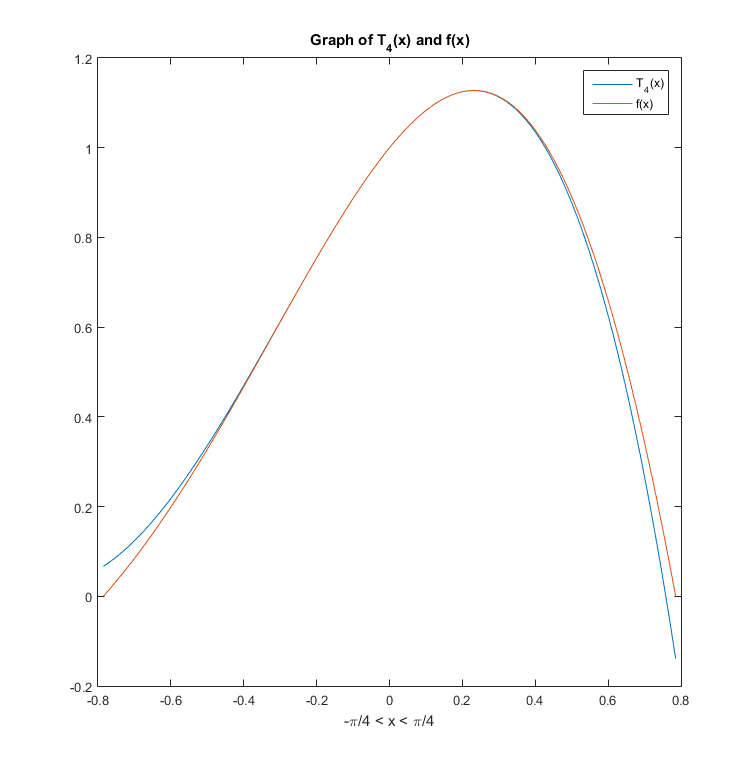
\includegraphics[width=4in, height=3.5in]{tf.png}
	\caption{Taylor expansion and initial function}
	\label{fig:graph1}
\end{figure}

\begin{figure}[!h]
	\centering
	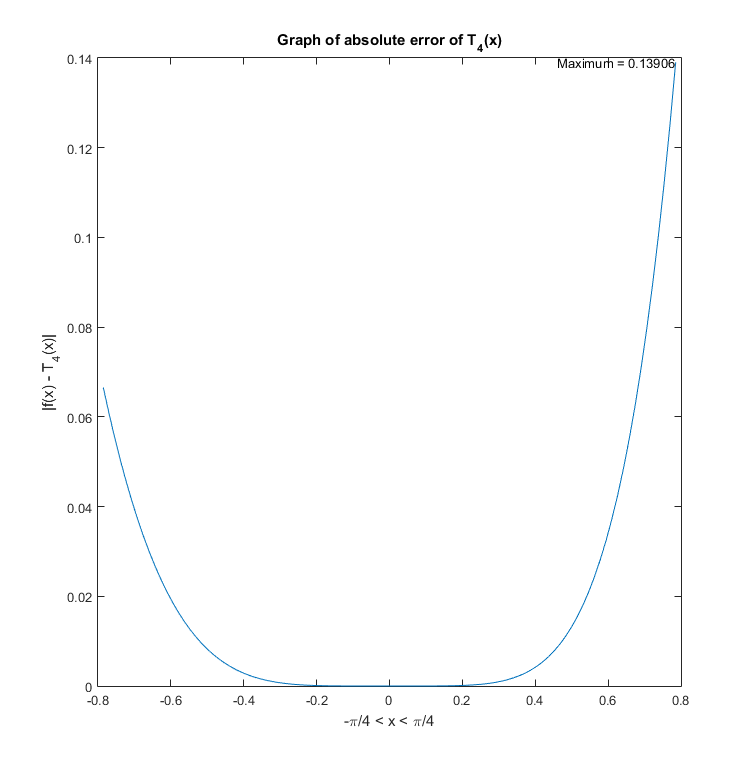
\includegraphics[width=4in, height=3.5in]{abs_error.PNG}
	\caption{Difference between the Taylor expansion and the initial function}
	\label{fig:graph2}
\end{figure}

\eenum

% Problem 2
\item

	$b = 10.\overline{110}_2$
	$= 2^1 + (0.\overline{110})_2$

	$z = 0.\overline{110}_2$

	$z = 0.110\overline{110})2$

	$2^3*z = 110.\overline{110}_2 = 2^2 + 2^1 + z$

	$8z = 6+z$

	$z = \frac{6}{7}$

	$b_{10} = 2 + z_{10} = 2 + \frac{6}{7} = \frac{18}{7} = 2.\overline{857142}$

% Problem 3
\item


	$6.7_{10}$

	$6_{10} = 110_2$

	\begin{tabular}{ll}

		$\frac{14}{10} = d_1 + \frac{d_2}{2} + \cdots$ & $ d_1 = 1$ \\

		$\frac{4}{5} = d_2 + \frac{d_3}{2} + \cdots$ & $d_2 = 0$ \\

		$\frac{8}{5} = d_3 + \frac{d_4}{2} + \cdots$ & $d_3 = 1$ \\

		$\frac{6}{5} = d_4 + \frac{d_5}{2} + \cdots$ & $d_4 = 1$ \\

		$\frac{2}{5} = d_5 + \frac{d_6}{2} + \cdots$ & $d_5 = 0$ \\

		$\frac{4}{5} = d_6 + \frac{d_7}{2} + \cdots$ & $d_6 = 0$ \\

	\end{tabular} \\

	The value generating $d_6$ is the same as the one generating $d_2$, and thus we are in a loop generating
	the repeating pattern 0110.

	$6.7_{10} = 110.1\overline{0110}_2 = 1.101\overline{0110}*2^2$

	The IEEE representation of this number designates one signed bit (in this case it is 0, as 6.7>0), 8 for the exponent (in this case 2),
	and 23 for the mantissa (in this case $101\overline{0110}$. The $23^{rd}$ digit of the mantissa is 0, so the number is truncated when
	stored.

	The exponent that is stored is the real exponent + a bias, which in this case is 127.

	$fl(6.7)$ is stored in the machine as

	\begin{center}
	\begin{tabular}{c | c | c}

		$0$ & $10000001$ & $10101100110011001100110$ \\

		sign & exponent + bias & mantissa \\

	\end{tabular} \\
	\end{center}

	Converting the stored number back to decimal gives us $2^{129-127} * q$

	$q = 1 + 2^{-1} + 2^{-3} + 2^{-5} + 2^{-6} + 2^{-9} + 2^{-10} + 2^{-13} + 2^{-14} + 2^{-17} + 2^{-18}+2^{-21} + 2^{-22} \approx 1.675$

	$fl(6.7) = 2^2 * q  \approx (6.7+1.90735*10^{-7})$

	The relative error $d = \frac{6.7-fl(6.7)}{6.7} = 2.84679*10^{-8}$

	$\epsilon_{mach}$ for a 32 bit float is $\frac{1}{2^{23}} \approx 1.19*10^{-7}$

	$\frac{1}{2} * \epsilon_{mach} \approx 5.96 * 10^{-8}$

	Crucially, $$\frac{1}{2} * \epsilon_{mach} \leq d$$ \\

% Problem 4
\item Holmes 1.5

\benum

	\item According to the IEEE double precision standard, $16_{10}$ is stored as

	$1*2^{5} =$

	\begin{center}
	\begin{tabular}{c | c | c}

		$0$ & $10000000100$ & $0\cdots0$ \\

		sign & exponent + bias of 1023 & 52 bit mantissa \\

	\end{tabular} \\
	\end{center}

	If we let $d_n$ represent the $n^{th}$ digit in the mantissa, then the last digit stored in the machine is $d_{52}=0$. By using
	the round-to-nearest rule, if $d_{53}$ is a 1, we increment $d_{52}$ by one, then chop. This, however, would change the value of the
	stored number. If $d_{53}$ is 0, however, the number is simply chopped after $d_{52}$ with no modifications. In other words, if
	$d_1 d_2 \cdots d_{52} d_{53} ==  0$, then $d_{54} d_{55} \cdots d_{\infty}$ can take any value they like. More importantly, the
	upper bound of this value is when $d_{54} = d_{55} = \cdots = d_{\infty} = 1$

	$$d_{54} d_{55} \cdots d_{\infty} = \sum_{i=54}^{\infty}2^{-i} = \frac{1}{9007199254740992} \approx 1.11*10^-16$$
	This makes the upper bound of 16 $R=16+\frac{1}{9007199254740992} \approx 16.000000000000000111$ \\

	The lower bound of 16 can be done by finding the lowest value at which $15.xxx$ rounds up to 16. In order to round up at all using
	the round-to-nearest rule, we know that $d_{53}$ of $15.xxx$ must be a 1. This will cause $d_{52}$ to increase by 1, and the number
	will then be chopped. In order for the entire sequence $d_1 d_2 \cdots d_{52}$ to go to zeros, they must initially all be 1, and the
	overflow will convert $15.xxx$ into $16.000\cdots$, as well as increase the exponent.
	This value would therefore be stored as \\

	\begin{center}
	\begin{tabular}{c | c | c}

		$0$ & $10000000010$ & $1\cdots1$ \\

		sign & exponent + bias of 1023 & 52 bit mantissa \\

	\end{tabular} \\
	\end{center}

	In this case, the values of $d_{54} d_{55}
	\cdots d_{\infty}$ are arbitrary, and their lower bound would be $d_{54} = d_{55} = \cdots = d_{\infty} = 0$. So, the lowest value we
	can take is
	$$L=15+\sum_{i=1}^{53}2^i = \frac{144115188075855871}{9007199284740992} \approx 15.99999999999999989$$

	\item The same process can be used to find the upper and lower bounds of 50, but is slightly altered because of the IEEE
	representation.

	The upper bound is found the exact same way.
	$$R = 50 + \sum_{i=54}^{\infty}2^{-i} = \frac{450359962737049601}{9007199254740992} \approx 50.000000000000000111$$

	However, the lower bound is slightly altered, due to the binary form of 50.

	$50 = 110010 = 1.1001*2^5$ \\

	\begin{center}
	\begin{tabular}{c | c | c}

		$0$ & $10000000100$ & $10010\cdots0$ \\

		sign & exponent + bias of 1023 & 52 bit mantissa \\

	\end{tabular} \\
	\end{center}

	Here, the lower bound would be $49.xxx$, where all decimal places in the binary form are 1, through the same logic as part(a). \\

	\begin{center}
	\begin{tabular}{c | c | c}

		$0$ & $10000000100$ & $100011\cdots1$ \\

		sign & exponent + bias of 1023 & 52 bit mantissa \\

	\end{tabular} \\
	\end{center}

	Only the values of $d_6$ through $d_{52}$ can be set to 1, as any other modifications would not represent the number $49.xxx$.
	Because of this, the lower bound is
	$$L = 49 + \sum_{i = 1}^{46}2^{-i} = \frac{3518437208883199}{70368744177664} \approx 49.999999999999985$$

\eenum

% Problem 5
\item

	\begin{figure}[h!]
		\centering
		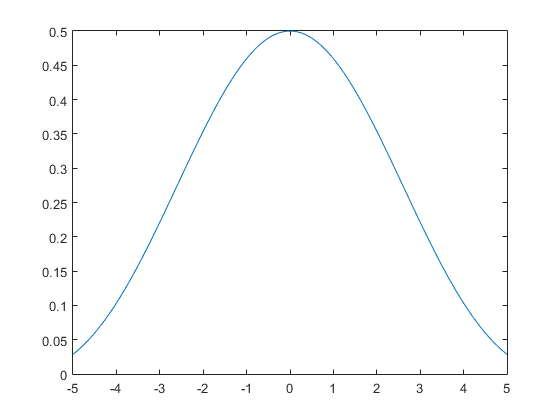
\includegraphics[width=4in, height=3.5in]{holmes1_12.png}
		\caption{Graph of $\frac{1-cos(x)}{x^2} $}
		\label{fig:graph333}
	\end{figure}

	It is known that $cos(0) = 1$, so as $x \rightarrow 0^+$, the numerator of this function becomes extremely small. When the machine
	subtracts these two quantities, there is a point at which catastrophic collision begins, which introduces significant error. When the
	number of ones in the binary form of $cos(x)$ is greater than 52 (the maximum number of digits in an IEEE double precision number),
	the result will dip below the underflow limit and is seen by the machine as zero.
	$$cos(10^{-8}) \approx 0.9999999999999999_{10} \approx 0.111\cdots101_2$$
	At $x=10^{-8}$, there are 54 leading ones in the binary form of $cos(x)$, so the machine computes the numerator as zero. The
	denominator, however, can still be accurately computed as $x^2$, so the result is simply 0.
	At slightly
	larger values of x ($x=10^{-7}$), there are less than 52 ones, so the machine can still do meaningful subtraction, albeit with minimal
	significance in the result.

% Problem 6
\item
Assume single-precision IEEE arithmetic. Assume that the round-to-nearest rule is used with one modification: if there is a tie then the smaller value is picked (this rule for ties is used to make the problem easier).
\benum
\item
	In order for $x>1$ to hold, the machine must see $x$ as at least $1+\epsilon_{mach}$. For a single precision machine, $\epsilon_{mach}
	=\frac{1}{2^{23}} \approx 1.19*10^{-7}$. We must now find the lowest possible value of $x$ needed for the machine to make the
	assignment. According to the round to nearest rule, a float will be rounded up if the binary representation of $x$ has a 1 in the
	$24^{th}$ decimal place, and digits $[25, \infty)$ hold at least one nonzero digit. The smallest binary value of $x$ that satisfies
	these requirements is $$x_1 = 1.000\ 000\ 000\ 000\ 000\ 000\ 000\ 001\ 0\cdots1_2$$
	As this number contains an infinite number of zeros after between the final two ones, we can only say that $x$ must be greater
	than $x^*$. Therefore,
	$$x>1+2^{-24} \rightarrow x>1.000000059604644775390625$$\\

	In order for $x<2$ to hold, the machine must see $x$ as at most $2-\epsilon_{mach}$. The maximum possible value of $x$ that is seen
	as $2-\epsilon_{mach}$ is the upper bound on the inequality. According to the round to nearest rule, a float will be rounded down if
	the final digit in the binary representation of $x$ has a 1 in the $24^{th}$ decimal place, and digits $[25, \infty)$ are all zero.
	This is the maximum possible value that can be rounded down, which can be written as
	$$x_2 = 2-2^{-24} = 1.999999940395355224609375$$
The values for which $1<x<2$ will hold on a single precision machine are $$(1.000000059604644775390625, 1.999999940395355224609375]$$ \\

\item
	In order for $x=4$ to hold, $x$ must be within the machine's ``margin of error'', or within $\pm \epsilon_{mach}$. According to the
	round to nearest rule, the machine will round up if the float's binary representation has a 1 in the $24^th$ decimal place, and digits
	$[25, \infty)$ hold at least one nonzero digit. The minimum possible value of $x$ that the machine will store as 4 is then

	$x_1 > (4-2^{-24}) \rightarrow x_1 > 3.999999940395355224609375$. \\

	The maximum possible value of $x$ that the machine will store as 4 would simply be $4+2^{-24}$, as a 1 in the $24^{th}$ decimal place
	of the binary representation, followed by all zeros is rounded down.

	$x_2 = 4+2^{-24} \rightarrow x_2 < 4.000000059604644775390625$.

	$$x_1 < x < x_2 \rightarrow x=4$$ \\

\item

	This number is not possible because $\sqrt{2}$ is irrational, so it containts an infinite number of nonrepeating decimal digits.
	Because machines are finite precision, no computer can fully represent $\sqrt{2}$ without any rounding or approximation. \\

	When converted to binary, $\sqrt{2}_2 = 1.011\ 010\ 100\ 000\ 100\ 111\ 100\ 11\cdots$. Therefore, $x^*_l$ is the truncated form
	of the number, and $x^*_r$ the truncated form of $\sqrt{2} + 2^{-23}$

	$$x^*_l = 1.011\ 010\ 100\ 000\ 100\ 111\ 100\ 11,\ x^*_r = 1.011\ 010\ 100\ 000\ 100\ 111\ 101\ 00$$

	\begin{center}
	\begin{tabular}{cc}
		&$1.01101010000010011110100$ \\
		$-$ & $1.01101010000010011110011$ \\
		\hline
		&$0.00000000000000000000001$ \\
	\end{tabular}
	\end{center}

	$$x^*_r - x^*_l = 2^{-23} = 1.1920928955078125×10^-7$$ \\

\eenum

% Problem 7
\item
\benum
\item A problem is ill-conditioned if its solution is highly sensitive to small changes in the input data.  True or False? \\
	True. An ill-conditioned problem will grow a slight error in input data to a large error in later stages \\

\item Using higher-precision arithmetic will make an ill-conditioned problem better conditioned.  True or False? \\
	False. While the initial input data may not be as incorrect, an ill-conditioned problem will still grow that error until the result
	is not significant. \\

\item  If two real numbers are exactly representable as floating-point numbers on a finite-precision machine, then so is their product.  True or False? \\
	False. If the two numbers are small enough, i.e. $2^-{23} * 2^{-23}$ on a single-precision machine, then their product will be
	smaller than the underflow limit of the machine, which cannot be exactly represented.
\item  Consider the sum
\[
S = \frac{1}{x+1} + \frac{1}{x-1}, \quad x \ne 1.
\]
For what range of values is it difficult to compute $S$ accurately in a finite-precision system?  How will you rearrange the terms in $S$ so that the difficulty disappears?
\item In a finite-precision system with UFL = $10^{-40},$ which of the following operations will incur an underflow?
\benum
\item $\sqrt{a^2+b^2},$ with $a=1, \; b=10^{-25}.$
\item $\sqrt{a^2+b^2},$ with $a=b=10^{-25}.$
\item $(a\times b)/(c \times d),$ with $a=10^{-20}, \; b=10^{-25}, \; c=10^{-10}, \; d=10^{-35}.$
\eenum

\eenum

\eenum
\end{document}
